\documentclass{article}
\usepackage{graphicx}
\usepackage{amsmath}
\usepackage{amssymb}
\usepackage{amsthm}
\usepackage{booktabs}
\usepackage{graphicx}

\usepackage[margin=1in]{geometry}

\newcommand{\Pois}{\mathrm{Pois}}
\newcommand{\Normal}{\mathcal{N}}
\newtheorem{proposition}{Proposition}[section]
\numberwithin{equation}{section}

\title{\textbf{Weighted Adaptive Conformal Prediction under Covariate Shift for Time Series}}
\author{Andrew Lou \and Shuyi Wang \and Zhimei Ren}
\date{}

\begin{document}

\maketitle

\begin{abstract}
We consider the problem of constructing prediction bands for time series data when the exchangeability assumption between training and testing data no longer holds due to covariate shift. We propose an algorithm that combines Adaptive Conformal Inference (ACI) with a likelihood-ratio-weighted conformal component, where the likelihood ratio is estimated via a logistic classifier. The adaptive component provides long-run coverage guarantees regardless of classifier accuracy, while the weighting component improves efficiency (band width) when the shift is well-estimated. This technical note presents the problem setup, the proposed algorithm, preliminary theoretical observations, and the experimental design for preliminary empirical evaluation.
\end{abstract}

\section{Introduction}

Standard split conformal prediction assumes that calibration and test data are exchangeable, an assumption that fails in time series settings where distributional characteristics may shift between training and deployment. Two existing lines of work address this limitation. Adaptive Conformal Inference (ACI) adjusts the nominal miscoverage level online based on observed coverage errors, correcting for shift after the fact (Gibbes and Candes, 2021). Weighted conformal prediction reweights calibration scores by the likelihood ratio between test and calibration covariate distributions, exploiting structural knowledge of the shift (Tibshirani et al, 2018). 

In this note, we propose an algorithm that combines both approaches. The likelihood ratio is estimated by training a logistic classifier to discriminate calibration from test samples. The adaptive component handles residual miscoverage when the classifier is imperfect, while the weighting component sharpens the prediction band when the shift is well-characterized. We view this decoupling as the central contribution: the weights shape the calibration distribution, and the adaptive update corrects the level.

\subsection{Use-case:}
Autonomous systems must make sequential decisions in environments whose future evolution is only partially predictable. For example, an autonomous vehicle or mobile robot may rely on a learned trajectory forecaster to predict the future positions of nearby pedestrians, cyclists, or vehicles before selecting a safe path. Calibration data are often collected in a limited set of environments, while deployment may occur under different traffic density, road geometry, lighting, weather, or behavioral regimes. In such settings, the observable trajectory state distribution can shift substantially between calibration and deployment, even when the short-horizon conditional dynamics given the observed state remain similar. A conformal method for covariate-shifted trajectories is therefore useful because the planner needs prediction bands that are wide enough to remain safe under shifted scene conditions, but not so conservative that the robot becomes unnecessarily immobilized.

Power-system operators and energy-market participants also rely on sequential forecasts whose errors have operational consequences. Day-ahead and intraday forecasts of electricity prices, load, wind generation, or solar production inform reserve procurement, storage dispatch, congestion management, and market bidding. These time series are naturally nonstationary: the distribution of observable forecasting states can change across seasons, renewable penetration regimes, demand regimes, weather regimes, and market locations. A conformal method that uses target-period covariates to reweight calibration errors, while retaining online adaptive correction, is attractive in this setting because ordinary calibration data may overrepresent normal operating conditions and underrepresent precisely the high-load or high-renewable regimes in which uncertainty estimates are most consequential.

\subsection{Related Literature}

Conformal prediction provides distribution-free predictive inference under
exchangeability, converting an arbitrary point predictor or score function into
prediction sets with finite-sample marginal coverage. This framework has been
developed extensively for regression, classification, and related prediction
tasks; see Vovk, Gammerman, and Shafer (2005), Lei et al. (2018), and related
work. A central limitation, however, is that the standard coverage guarantee
requires the calibration and test observations to be exchangeable. This
assumption is often violated in time-series deployment and in source-to-target
transfer settings.

A first line of work studies conformal prediction under covariate shift.
Tibshirani et al. (2019) show that when the covariate distribution changes from
a source law \(P_X\) to a target law \(\widetilde P_X\), while the conditional
response law \(P_{Y\mid X}\) remains invariant, conformal validity can be
restored by replacing the ordinary empirical quantile of calibration scores with
a likelihood-ratio-weighted quantile. Their theory is exact when the density
ratio \(d\widetilde P_X/dP_X\) is known, and they also discuss estimating this
ratio from unlabeled target covariates using probabilistic classifiers. This
work gives the statistical foundation for reweighting calibration scores, but it
is primarily formulated for static prediction rather than online trajectory
forecasting.

A second line of work addresses non-exchangeability and temporal distribution
shift through adaptive conformal methods. Gibbs and Candès (2021) introduce
adaptive conformal inference (ACI), which updates the nominal miscoverage level
online based on past coverage errors. Their method achieves long-run empirical
coverage under arbitrary distribution shifts, without assuming exchangeability
of the sequence. Gibbs and Candès (2024) further develop online conformal
procedures with stronger local adaptivity by tuning the update step size over
time. Angelopoulos, Candès, and Tibshirani (2023) connect this line of work to
control-theoretic ideas through conformal PID control, yielding online conformal
methods that adapt to systematic errors arising from seasonality, trends, and
other forms of distribution shift. These methods are robust and online, but they
do not directly exploit unlabeled target covariates to correct calibration
scores before deployment errors are observed.

A third line of work focuses specifically on conformal inference for time
series. Xu and Xie (2021) propose EnbPI, a bootstrap-ensemble conformal method
for sequential prediction intervals with approximate validity under broad
classes of dependent time-series errors. Xu and Xie (2023) propose sequential
predictive conformal inference (SPCI), which adaptively estimates conditional
quantiles of future nonconformity scores using temporal dependence. Stankeviciute,
Alaa, and van der Schaar (2021) extend inductive conformal prediction to
multi-horizon time-series forecasting with recurrent predictors. These methods
address temporal dependence and sequential forecasting, but they do not target
the source-to-target covariate-shift setting in which calibration trajectories
and deployment trajectories are drawn from different covariate distributions.

A related trajectory-level literature studies simultaneous coverage for entire
forecast paths. Zhou, Lindemann, and Sesia (2024) propose conformalized adaptive
forecasting of heterogeneous trajectories (CAFHT), combining ideas from online
conformal prediction and multi-series conformal calibration to produce
simultaneous forecasting bands for a new trajectory. Their method is designed to
handle heterogeneous trajectory difficulty and provides finite-sample
simultaneous marginal coverage under exchangeability of calibration and test
trajectories. The present work builds on this perspective but considers a
different deployment regime: the target trajectories may have a shifted
covariate distribution relative to the calibration trajectories.

Other work has considered broader departures from exchangeability. Barber et al.
(2023) develop conformal prediction beyond exchangeability, using weighted
quantiles and randomized constructions to reduce coverage degradation under
distribution drift and nonsymmetric algorithms. Cauchois et al. (2024) study
robust validation, constructing prediction sets with coverage over classes of
test distributions lying in an \(f\)-divergence neighborhood of the training
distribution. Podkopaev and Ramdas (2021) study distribution-free uncertainty
quantification under label shift, showing how reweighting can restore coverage
and calibration in classification when unlabeled target data are available.
These papers demonstrate the broader importance of distribution shift for
uncertainty quantification, but they do not provide a method specialized to
covariate-shifted online trajectory prediction.

Our contribution lies at the intersection of these strands. We study
multi-series time-series prediction under covariate shift, where source
calibration trajectories and target deployment trajectories need not be
exchangeable but the conditional response law is assumed stable given the
observed forecasting state. We combine likelihood-ratio-weighted conformal
calibration, which uses target covariate information before deployment, with
adaptive conformal updates, which correct residual miscoverage after outcomes
are observed. This combination addresses a gap between weighted conformal
methods for static covariate shift, adaptive conformal methods for online
distribution shift, and trajectory-level conformal methods that assume
exchangeable trajectories.


\section{Problem Statement and Notation}

Consider a data set $\mathcal{D}$ with $n$ array observations each of length $T+1$, where the $i$-th observation is denoted $\mathbf{Y}^{(i)}$ for $i = 1, \ldots, n$. Each observation $\mathbf{Y}^{(i)}$ can be represented as $(Y^{(i)}_0, Y^{(i)}_1, \ldots, Y^{(i)}_T)$, where $Y^{(i)}_t$ is a $d$-dimensional vector measured at time step $t$.

We would like to construct an informative prediction band that covers $\mathbf{Y}^{(n+1)}$ with pre-specified probability. Instead of assuming that $\mathbf{Y}^{(n+1)}$ is sampled exchangeably from the same distribution as $\mathcal{D}$, we assume a setting where a covariate shift occurs. That is, we observe data according to:
\begin{equation} \label{eq:1}
\begin{gathered}
(\mathbf{Y}^{(i)}_{0 \ldots T-1}, Y^{(i)}_T) \overset{\mathrm{iid}}{\sim} P = P_{\mathbf{Y}_{0 \ldots T-1}} \times P_{Y_T \mid \mathbf{Y}_{0 \ldots T-1}}, \quad i = 1, \ldots, n \\
(\mathbf{Y}^{(n+1)}_{0 \ldots T-1}, Y^{(n+1)}_T) \overset{\mathrm{iid}}{\sim} \widetilde{P} = \widetilde{P}_{\mathbf{Y}_{0 \ldots T-1}} \times P_{Y_T \mid \mathbf{Y}_{0 \ldots T-1}}, \text{ independently}
\end{gathered}
\end{equation}
Henceforth, we denote $P_{\mathbf{Y}_{0 \ldots T-1}}$ and $\widetilde{P}_{\mathbf{Y}_{0 \ldots T-1}}$ as $P_Z$ and $\widetilde{P}_Z$, respectively, for simplicity of notation. The difference between $P_Z$ and $\widetilde{P}_Z$ constitutes the covariate shift.

\section{Method}

\subsection{Weighted Conformal Score}

For a time series $i$, we use an error term $\epsilon_i$ as a conformal score. $\epsilon_i$ is $\hat{C}(\mathbf{Y}^{(i)}, \gamma)$'s largest margin of error observed over the entire time series. That is, if the prediction band $\hat{C}(\mathbf{Y}^{(i)}, \gamma)$ is expanded by $\epsilon_i$ on both sides, the entire time series $i$ would be exactly covered by the adjusted prediction band.

Typical conformal prediction assumes the empirical distribution of conformal scores remains the same between training and testing data. Under a covariate shift, we adapt the conformal prediction process by weighting each conformal score proportionally to the likelihood ratio $w(i) = d\widetilde{P}_Z(i) / dP_Z(i)$.

Formally, an unweighted empirical distribution can be expressed as
\begin{equation} \label{eq:2}
\frac{1}{n+1} \left( \sum^n_{i=1} \delta_{\epsilon_i} + \delta_\infty \right),
\end{equation}
where $\delta_a$ denotes a point mass at $a$. The weighted empirical distribution can be expressed as
\begin{equation} \label{eq:3}
\sum^n_{i=1} p_i(z) \delta_{\epsilon_i} + p_{n+1}(z) \delta_\infty,
\end{equation}
where
\begin{equation} \label{eq:4}
p_i(z) = \frac{w(i)}{\sum_{j=1}^{n+1} w(j)}.
\end{equation}

\subsection{Weighted CAFHT}

Our main proposal combines CAFHT (adapted to our setting) with a likelihood-ratio classifier for online deployment. The likelihood ratio classifier is trained by labeling training samples as class $0$ and held-out test samples as class $1$; the resulting logistic classifier provides an estimate of $w(i) = d\widetilde{P}_Z / dP_Z$.

\begin{table}[t]
\centering
\caption{Online weighted CAFHT procedure.}
\label{alg:main}
\begin{minipage}{0.94\linewidth}
\small
\textbf{Input:} Desired error level $\alpha \in (0,1)$, training set $\mathcal{D}_{tr}$, calibration set $\mathcal{D}_{cal}$, test set $\mathcal{D}_{test}$, and learning-rate grid $\Gamma = \{0.001, 0.005, 0.01, 0.05, 0.1\}$.\\[0.5ex]
\textbf{Output:} Online prediction bands $\hat{C}(\mathbf{Y}^{(i)})$ for all $i \in \mathcal{D}_{test}$.\\[0.75ex]
\textbf{Procedure:}
\begin{enumerate}
    \item For each $t \in [T]$, train the predictor using $\{Y_j^{(i)} : j \in [t],\; i \in \mathcal{D}_{tr}\}$.
    \item Every 10 time steps, split $\mathcal{D}_{tr}$ into $\mathcal{D}_{tr}^{(1)}, \mathcal{D}_{tr}^{(2)}, \mathcal{D}_{tr}^{(3)}$ and evaluate each $\gamma \in \Gamma$ by running simple ACI on this three-way split up to time $t$; set $\gamma_{\mathrm{opt}}$ to the best-performing step size.
    \item Split the test set into two halves, $\mathcal{D}_{test}^{(1)}$ and $\mathcal{D}_{test}^{(2)}$.
    \item Train a logistic classifier on $\{(Y_t^{(i)},0)\}_{i \in \mathcal{D}_{tr}} \cup \{(Y_t^{(i)},1)\}_{i \in \mathcal{D}_{test}^{(2)}}$ to estimate the likelihood ratio.
    \item Apply the classifier to $\{Y_t^{(i)}\}_{i \in \mathcal{D}_{cal}}$, obtain estimated likelihood ratios, and compute weighted conformity scores.
    \item Construct $\hat{C}_{t+1}(\mathbf{Y}^{(i)})$ with level $\alpha_{t+1}^{(i)}$ and step size $\gamma_{\mathrm{opt}}$ for all $i \in \mathcal{D}_{test}^{(1)}$.
    \item Swap the roles of $\mathcal{D}_{test}^{(1)}$ and $\mathcal{D}_{test}^{(2)}$, then repeat.
\end{enumerate}
\end{minipage}
\end{table}

We define the nominal levels
\[
\alpha_{t+1}^{(i)} := \alpha_t^{(i)} + \gamma \bigl( \alpha_t^{(i)} - err_t^{(i)} \bigr),
\]
where
\[
err_t^{(i)} :=
\begin{cases}
1, & \text{if } Y_t^{(i)} \notin \hat{C}_t(\mathbf{Y}^{(i)}), \\
0, & \text{otherwise}.
\end{cases}
\]

\section{Theoretical Properties}

Different methodologies target different performance metrics. Simple ACI provides a long-run coverage guarantee.

\begin{proposition}[Convergence for simple ACI]
With probability one, for all $T \in \mathbb{N}$,
\[
\left| \frac{1}{T} \sum_{t=1}^T err_t - \alpha \right|
\le
\frac{\max\{\alpha_1, 1 - \alpha_1\} + \gamma}{T \gamma}.
\]
In particular,
\[
\lim_{T \to \infty} \frac{1}{T} \sum_{t=1}^T err_t \overset{\text{a.s.}}{=} \alpha.
\]
\end{proposition}

A more sophisticated form of ACI targets entire-path coverage:
\[
\mathbb{P}\bigl[ Y_t^{(n+1)} \in \hat{C}_t(\mathbf{Y}^{(n+1)}), \; \forall t \in [T] \bigr] \ge 1 - \alpha.
\]

The details of the theoretical guarantee for our algorithm have yet to be finalized. We intend to craft the precise statement alongside the proof, and anticipate that long-run coverage is inherited from the ACI component irrespective of classifier accuracy, while the weighting component affects band width rather than coverage validity.

\section{Experiments}
\label{sec:experiments}

We evaluate Weighted CAFHT against two ablations on synthetic time series, S\&P~500 intraday returns, and medical data. All experiments set $\alpha = 0.10$ (target
coverage $1 - \alpha = 0.90$). Three algorithm variants are compared
throughout:
%
\begin{itemize}
  \item \textbf{Weighted CAFHT}: full method — likelihood-ratio (LR) covariate
        reweighting combined with per-series ACI $\alpha_t$ updating.
  \item \textbf{Uniform weights}: Logistic regression classifier (LR) weighting disabled (uniform calibration
        weights); per-series ACI update retained. Isolates the contribution of
        adaptive coverage correction.
  \item \textbf{Zero $\gamma$}: LR weighting enabled; ACI step size fixed at
        $\gamma = 0$ (no $\alpha_t$ update). Isolates the contribution of
        covariate reweighting.
\end{itemize}

\subsection{Synthetic Data}
\label{sec:experiments:synthetic}

\paragraph{Data-generating processes.}
We consider two synthetic DGPs, each generating $N_{\mathrm{train}} = 600$
training series, $N_{\mathrm{cal}} = 600$ calibration series, and
$N_{\mathrm{test}} = 300$ test series of length $T = 20$.

\textit{Static-X}: Each series is driven by a scalar covariate $X^{(i)}$
drawn once at series creation time.  Training and calibration covariates
follow $X \sim \mathrm{Pois}(\lambda)$ with $\lambda = 1$; under the
\emph{static shift} condition the test covariates are redrawn from
$\mathrm{Pois}(\tilde\lambda)$ with $\tilde\lambda = 2$.  Conditional on $X$,
the response follows an AR(1) process:
%
\[
  Y_t = \rho \, Y_{t-1} + \beta X + \delta t + \varepsilon_t, \quad
  \varepsilon_t \overset{\text{i.i.d.}}{\sim} \mathcal{N}(0, \sigma^2),
\]
%
with $\rho = 0.7$, $\beta = 1.0$, $\delta = 0$ (no deterministic drift), and
$\sigma = 0.2$.  Initial values are shared between train and test to hold
$Y_0$ fixed under shift.

\textit{Dynamic-X}: The covariate itself evolves as an AR(1):
$X_{t+1} = \rho_X X_t + \kappa_X t + \eta_t$, $\eta_t \sim \mathcal{N}(0,
\sigma_X^2)$.  Under the \emph{dynamic shift} condition the entire covariate
path is regenerated under shifted parameters $(\tilde\rho_X, \tilde\kappa_X,
\tilde\sigma_X)$, while $Y_0$ is held fixed.

\paragraph{Prediction model.}
At each time step $t$, an AR(1) model is fitted by OLS on all training
trajectories up to step $t$, producing point forecasts $\hat Y_{t+1}^{(i)}$.
The nonconformity score is the absolute residual
$s_t^{(i)} = |Y_t^{(i)} - \hat Y_t^{(i)}|$.

\paragraph{Likelihood-ratio estimation.}
For each time step the test set is split uniformly at random into two halves
$H_1, H_2$.  A logistic classifier with balanced class weights is fitted on
$\mathcal{D}_{\mathrm{train}} \cup H_2$ (labels $0/1$) and used to score
$H_1$, and vice versa.  This cross-half procedure prevents leakage of
deployment-distribution information into the calibration weights.
Estimated density ratios $\hat w(z) \propto \hat p(z) / (1 - \hat p(z))$ are
clipped at $5\times$ the mean weight and renormalized to sum to one.

\paragraph{ACI update and $\gamma$ selection.}
Each test series maintains its own coverage level $\alpha_t^{(i)}$, updated
after each observation via
%
\[
  \alpha_{t+1}^{(i)} = \alpha_t^{(i)}
    + \gamma \bigl(\alpha - \mathbf{1}\bigl[Y_{t+1}^{(i)} \notin
      \hat C_{t+1}^{(i)}\bigr]\bigr),
\]
%
clipped to $(10^{-6},\, 1 - 10^{-6})$.  The step size $\gamma$ is selected
every 10 steps by a held-out simulation on a three-way split of the training
data; the search grid is $\Gamma = \{0.001, 0.005, 0.01, 0.05, 0.1\}$.

\paragraph{Evaluation.}
Each configuration is replicated over 30 independent seeds (base seed 1000).
We report pooled empirical coverage (fraction of covered intervals across all
series and time steps), the mean per-seed absolute deviation
$\overline{|\Delta|} = \frac{1}{30}\sum_{s=1}^{30}
|\hat{\mathrm{cov}}_s - (1-\alpha)|$ from the target, and mean interval
width.


% ============================================================
%  TABLE 1: Synthetic Results
% ============================================================

\begin{table}[ht]
\centering
\small
\setlength{\tabcolsep}{8pt}
\renewcommand{\arraystretch}{1.15}
\caption{%
  Synthetic results ($T=20$, $\alpha=0.10$, 30 seeds, target coverage $= 0.90$).
  \textit{Coverage}: pooled empirical coverage across all series and time steps.
  $\overline{|\Delta|}$: mean per-seed absolute deviation from $1-\alpha$.
  \textit{Width}: mean prediction interval width.
}
\label{tab:synthetic}
\begin{tabular}{@{} llrrr @{}}
\toprule
{\bfseries Data condition} & {\bfseries Algorithm}
  & {\bfseries Coverage} & $\boldsymbol{\overline{|\Delta|}}$ & {\bfseries Width} \\
\midrule
No shift
  & Weighted CAFHT      & 0.901 & 0.001 & 1.395 \\
No shift
  & Uniform weights     & 0.901 & 0.001 & 1.394 \\
No shift
  & Zero $\gamma$       & 0.901 & 0.001 & 1.395 \\
\midrule
Static shift
  & Weighted CAFHT      & 0.891 & 0.009 & 1.501 \\
Static shift
  & Uniform weights     & 0.869 & 0.031 & 1.445 \\
Static shift
  & Zero $\gamma$       & 0.890 & 0.010 & 1.498 \\
\midrule
Dynamic shift
  & Weighted CAFHT      & 0.841 & 0.059 & 1.339 \\
Dynamic shift
  & Uniform weights     & 0.836 & 0.064 & 1.323 \\
Dynamic shift
  & Zero $\gamma$       & 0.838 & 0.062 & 1.332 \\
\bottomrule
\end{tabular}
\end{table}



\subsection{Results on S\&P 500 Stock Data}
\label{sec:experiments:finance}

\paragraph{Data.}
We use daily S\&P~500 intraday return data from 2024 collected via
\texttt{yfinance}.  The response variable is
$Y_t = \mathrm{Close}_t / \mathrm{Open}_t - 1$ for each ticker on each
trading day.  Four covariates are constructed for each ticker-day pair:
%
\begin{itemize}
  \item \textbf{OvernightGapReturn}: overnight return (not lagged).
  \item \textbf{Above52wLowReturn}: distance above the 52-week low, computed
        from pre-sample data to prevent lookahead bias (not lagged).
  \item \textbf{TurnoverRatio} (lagged one day).
  \item \textbf{DailyRangeReturn} (lagged one day).
\end{itemize}

\paragraph{Covariate shift design.}
We test two sector-based shift conditions.  In the first, the
\emph{Technology} sector forms the test set and the remaining $\sim\!480$
tickers provide the training and calibration pool.  In the \emph{Utilities}
setting, Utilities-sector tickers form the test set.  Sector membership is
fixed by GICS classification; the resulting covariate distributions differ
meaningfully from the pool (maximum Kolmogorov–Smirnov statistic $\approx
0.49$ for Technology, $\approx 0.75$ for Utilities, driven primarily by
beta-to-market features).  A \emph{Mixed} null baseline randomly draws 15\%
of all tickers as the test set, inducing no systematic sector shift.

The following diagnostic plots visualize the covariate shifts induced by using sector-specific test sets. They are intended to show that the Technology and Utilities test distributions differ meaningfully from the corresponding training and calibration pools before conformal calibration is applied.

\begin{figure}[!htbp]
\centering

\begin{minipage}[c][3.1in][c]{0.95\linewidth}
\centering

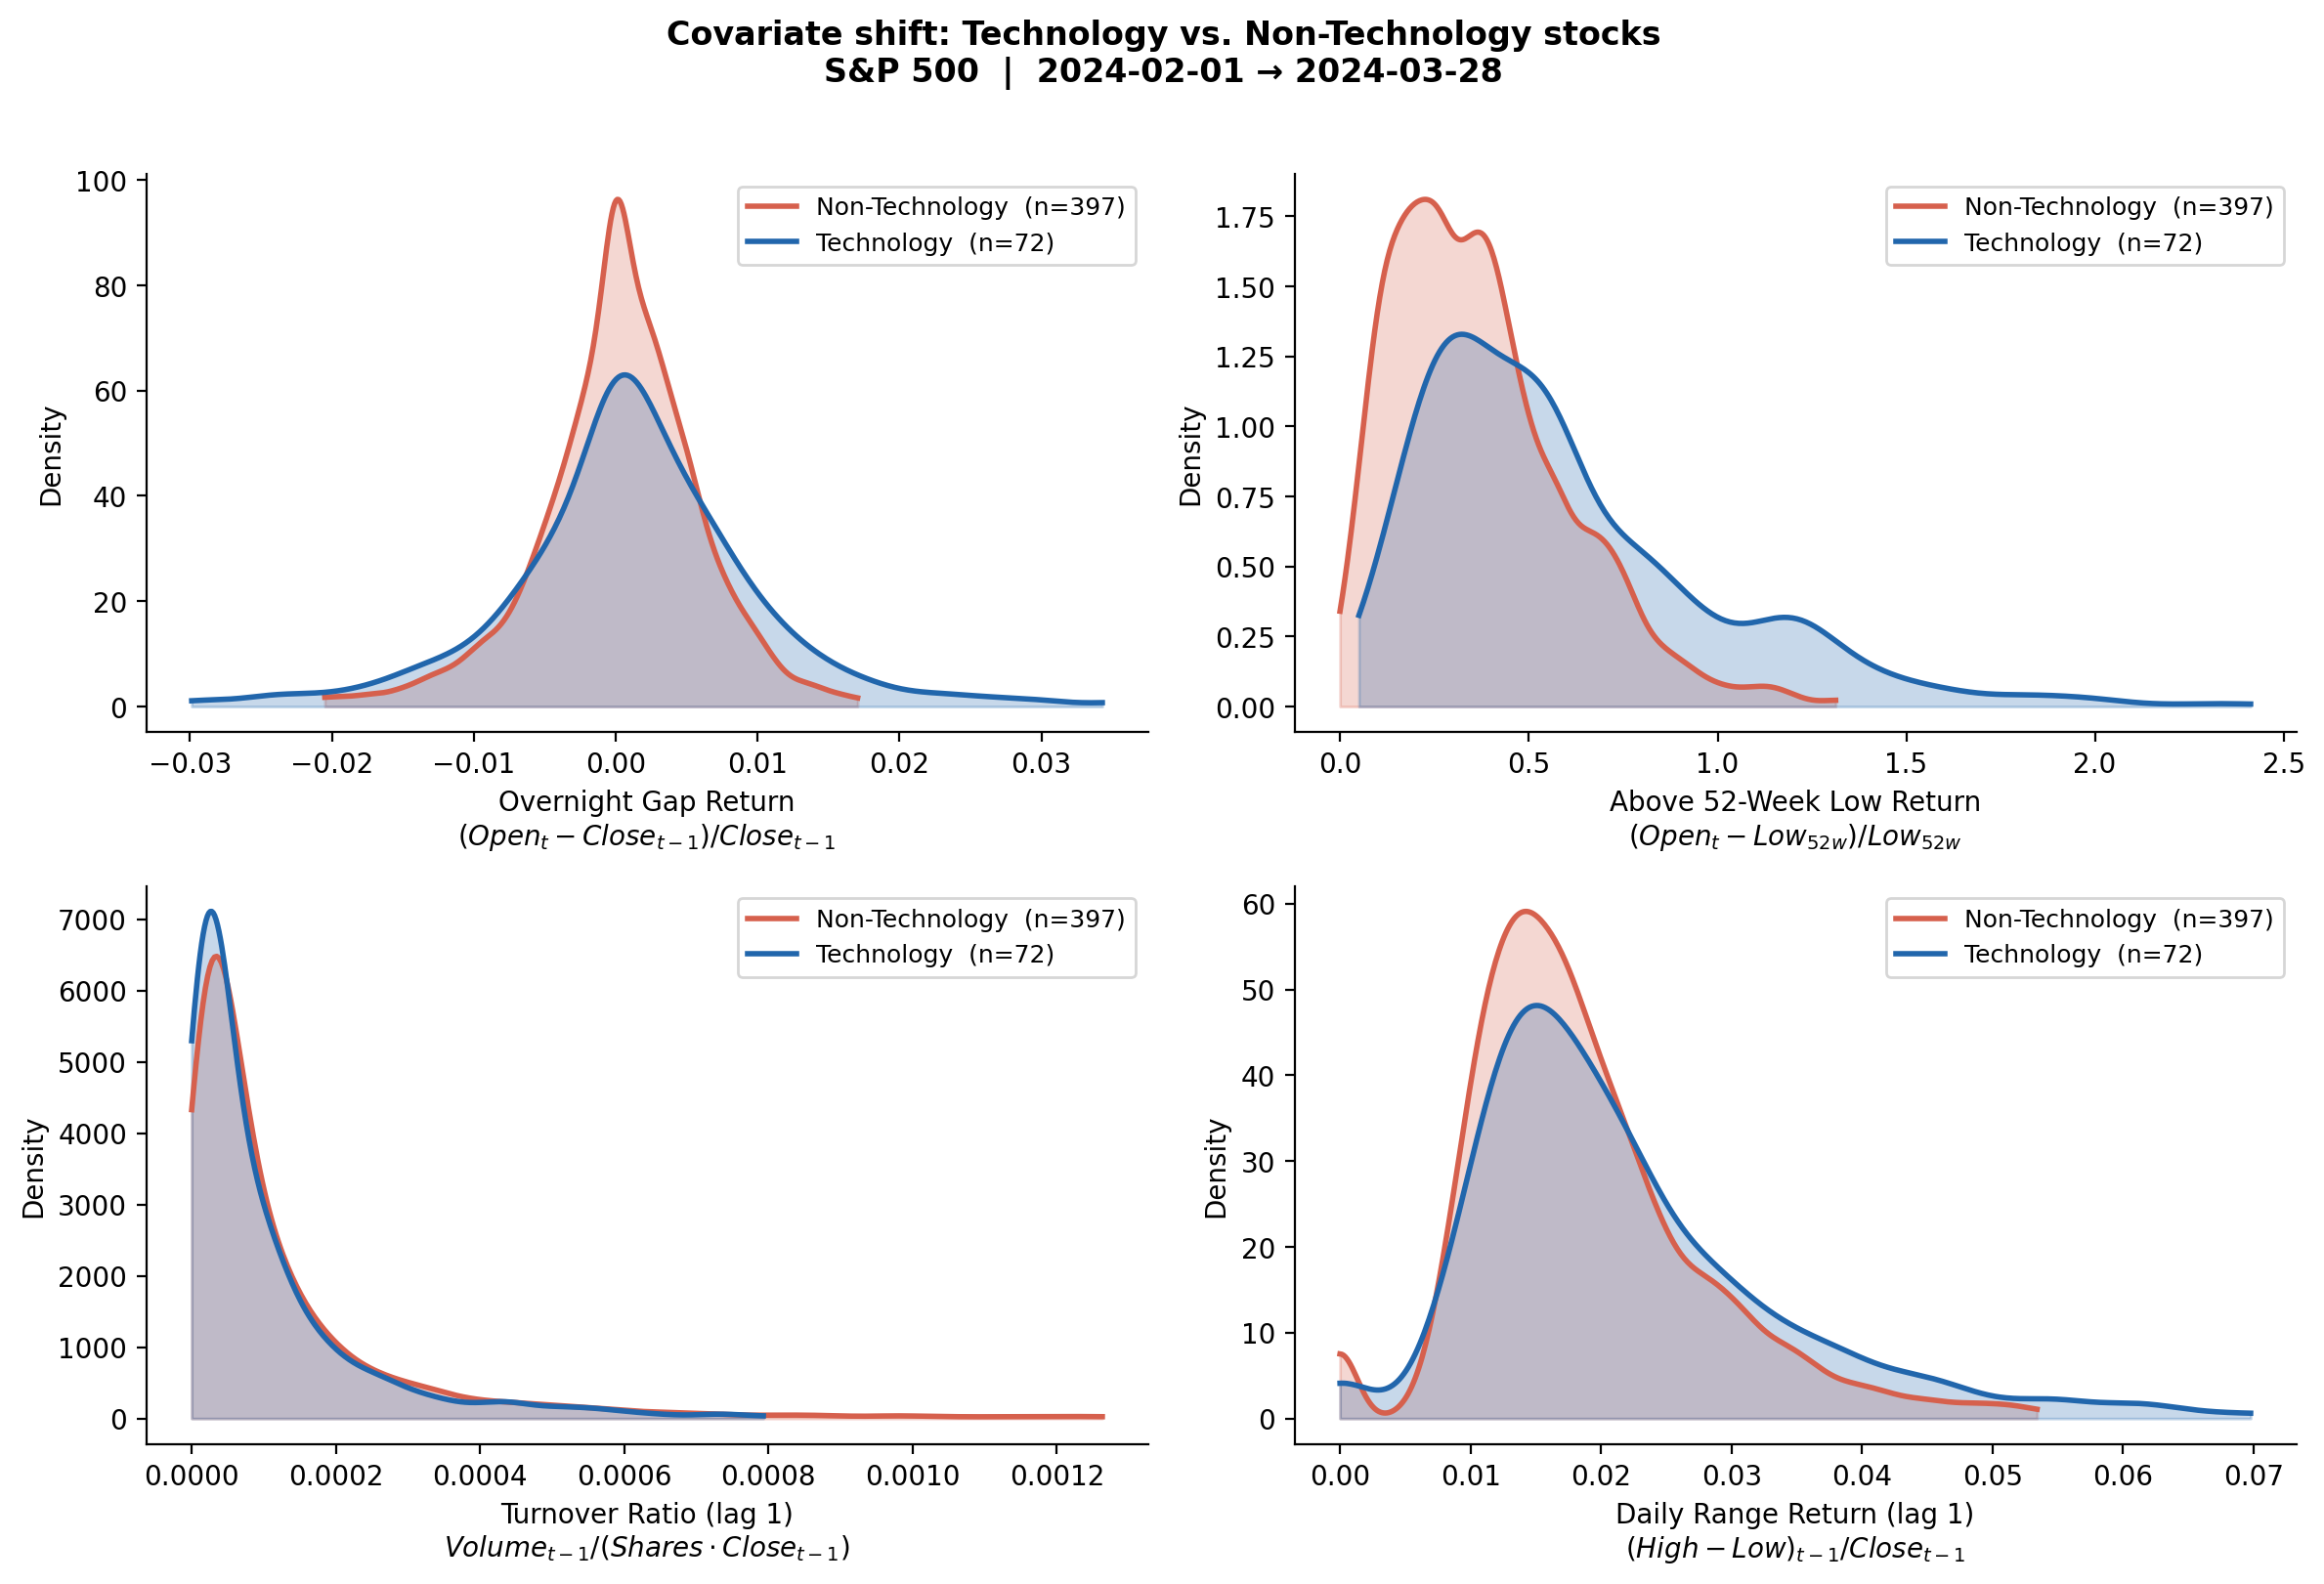
\includegraphics[
    width=\linewidth,
    height=3in,
    keepaspectratio
]{technology_shift.png}
\end{minipage}

\vspace{0.5em}

\begin{minipage}[c][3.1in][c]{0.95\linewidth}
\centering

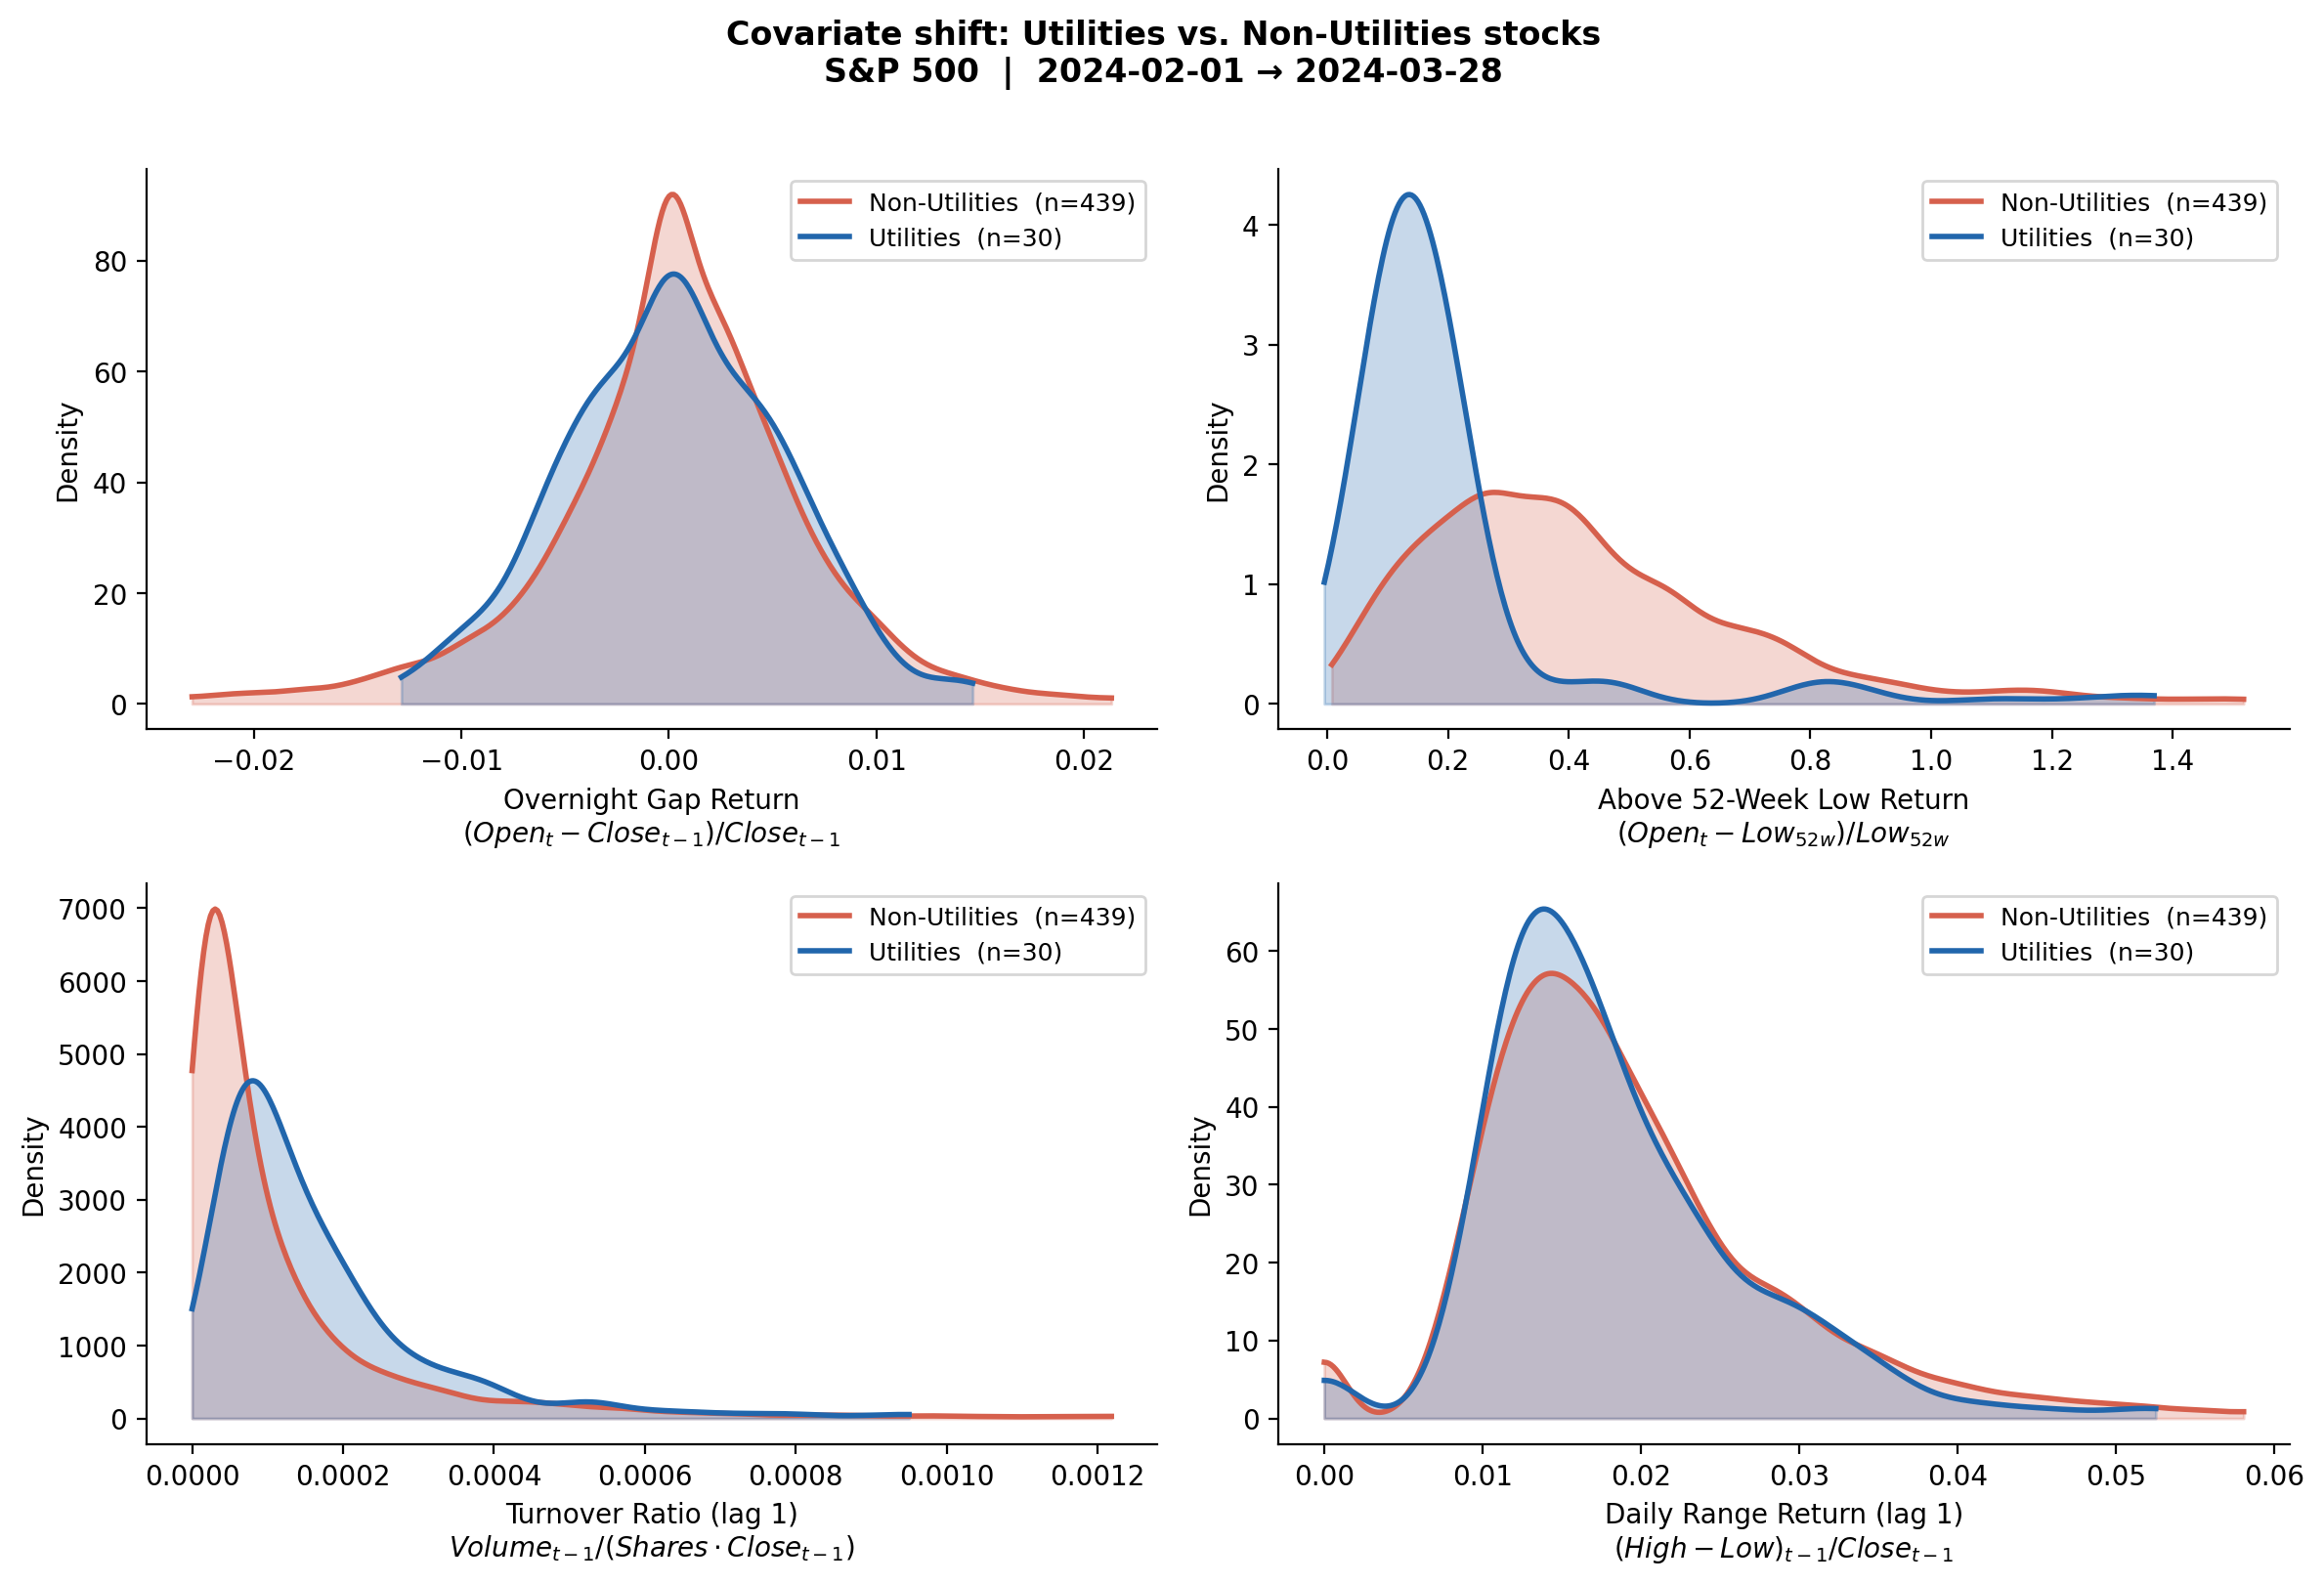
\includegraphics[
    width=\linewidth,
    height=3in,
    keepaspectratio
]{utilities_shift.png}
\end{minipage}

\caption{Covariate-shift diagnostics comparing Technology- and Utilities-sector test tickers against the training/calibration pool.}
\label{fig:finance-covariate-shift}
\end{figure}

\paragraph{Rolling windows and train/cal split.}
Experiments are run over 13 rolling two-month windows covering
January 2024 to March 2025.  Within each window, the non-test ticker pool is split
50/50 into training and calibration sets (seed 42).  The Technology and
Utilities conditions each yield 13 independent coverage observations; the
Mixed condition uses a single window.

\paragraph{Prediction model.}
At each time step $t$, an OLS regression of $Y$ on the four covariates is
fitted pooled across all training tickers and all time steps up to $t$,
producing ticker-level forecasts $\hat Y_{t+1}^{(i)}$.  The nonconformity
score is $s_t^{(i)} = |Y_t^{(i)} - \hat Y_t^{(i)}|$.

\paragraph{Likelihood-ratio estimation.}
The LR featurizer represents each ticker at time $t$ by: the mean, standard
deviation, and AR(1) coefficient of $Y$ over a rolling window of 10 steps,
together with the temporal mean and standard deviation of each of the four
covariates over the full prefix (11 features total).  As in the synthetic
setting, a cross-half logistic classifier estimates density ratios with
balanced class weights and $5\times$-mean clipping.

\paragraph{ACI update and $\gamma$ selection.}
The per-series ACI update is identical to the synthetic setting.  The search
grid is $\Gamma = \{0.001, 0.005, 0.01, 0.05\}$ for Technology and
$\Gamma = \{0.001, 0.005, 0.01, 0.05, 0.1\}$ for Utilities; $\gamma$ is
reselected every 10 steps.

\paragraph{Evaluation.}
For Technology and Utilities we report the mean per-window coverage and the
mean per-window absolute deviation $\overline{|\Delta|}$ from the target
$1-\alpha = 0.90$ averaged across the 13 windows.  Mean interval width is
reported in intraday return units.  The Mixed null baseline is reported for a
single window.
% ============================================================
%  TABLE 2: Finance Results
% ============================================================

\begin{table}[ht]
\centering
\small
\setlength{\tabcolsep}{8pt}
\renewcommand{\arraystretch}{1.15}
\caption{%
  Finance results (S\&P~500 intraday returns, $\alpha=0.10$, seed~42, target
  coverage $= 0.90$).
  Technology and Utilities: mean over 13 rolling windows.
  Mixed (null baseline): single window, 15\% random test draw.
  $\overline{|\Delta|}$: mean per-window absolute deviation from $1-\alpha$.
  \textit{Width}: mean interval width (intraday return units).
  Utilities uses $\gamma$-grid $\{0.001, 0.005, 0.01, 0.05, 0.1\}$;
  Technology uses $\{0.001, 0.005, 0.01, 0.05\}$.
}
\label{tab:finance}
\begin{tabular}{@{} llrrr @{}}
\toprule
{\bfseries Sector} & {\bfseries Algorithm}
  & {\bfseries Coverage} & $\boldsymbol{\overline{|\Delta|}}$ & {\bfseries Width} \\
\midrule
Technology
  & Weighted CAFHT      & 0.888 & 0.017 & 0.0505 \\
Technology
  & Uniform weights     & 0.880 & 0.024 & 0.0493 \\
Technology
  & Zero $\gamma$       & 0.872 & 0.029 & 0.0465 \\
\midrule
Utilities
  & Weighted CAFHT      & 0.923 & 0.026 & 0.0451 \\
Utilities
  & Uniform weights     & 0.924 & 0.027 & 0.0454 \\
Utilities
  & Zero $\gamma$       & 0.932 & 0.034 & 0.0447 \\
\midrule
Mixed (null)
  & Weighted CAFHT      & 0.911 & 0.011 & 0.0414 \\
Mixed (null)
  & Uniform weights     & 0.911 & 0.011 & 0.0413 \\
Mixed (null)
  & Zero $\gamma$       & 0.907 & 0.007 & 0.0417 \\
\bottomrule
\end{tabular}
\end{table}


\subsection{Results on Medical Data}
\label{sec:experiments:medical}

\paragraph{Data.}
We use the MIMIC-III Clinical Database (Johnson et al., 2016), a publicly
available de-identified electronic health record dataset of $\sim\!\!40{,}000$
ICU stays at the Beth Israel Deaconess Medical Center.  From this database we
extract a sepsis cohort of $15{,}091$ patients (ICD-coded sepsis diagnosis,
non-zero values across all four target variables for the full 24-hour window),
each represented by $T+1 = 24$ hourly observations beginning at ICU admission.
The response variable $Y_t$ is the patient's NaCl 0.9\% intravenous fluid
dosage (mL/hr) at hour $t$.  Three dynamic covariates are recorded at each
hour --- Heart Rate, Respiratory Rate, and O$_2$ saturation (pulse oximetry)
--- and six static covariates are recorded once per patient: age, a binary
gender indicator, and a four-level one-hot ethnicity encoding (Black,
Hispanic, Asian, Other; White is the reference category).  Following the
upstream extraction pipeline, all-zero covariate trajectories are excluded and
remaining intra-trajectory zeros in the dynamic covariates are imputed by the
patient's median nonzero value; zeros in the NaCl target are left unchanged.

\paragraph{Cohort and covariate-shift split.}
The covariate shift is induced by an exogenous treatment indicator,
Norepinephrine administration during the first twelve ICU hours.  Patients
who received \emph{no} Norepinephrine in hours $0$--$11$ form the
training/calibration pool ($n = 9{,}264$); patients who received
\emph{any} Norepinephrine in hours $0$--$11$ form the test pool
($n = 5{,}827$).  The two pools differ markedly in physiologic and
fluid-management state: the dominant marginal shift is in the NaCl target
itself (KL divergence Test\,$\|$\,TrainCal $\approx 0.206$), with smaller
shifts on O$_2$ saturation ($0.050$) and respiratory rate ($0.022$).
Because Norepinephrine timing is determined by clinical state rather than by
randomization, the resulting train/test partition is a natural covariate-shift
benchmark in which the conditional response law $P_{Y \mid Z}$ is plausibly
stable while the marginal distribution of $Z$ differs between source and
target populations.

\paragraph{Prediction model.}
At each hour $t$, a one-step-ahead OLS predictor of NaCl is fit pooled across
all training patients and all hours up to $t$:
\[
  \widehat{\mathrm{NaCl}}_{t+1}
  = \beta_0 + \beta_1 \mathrm{NaCl}_t + \beta_2 \mathrm{HR}_t
  + \beta_3 \mathrm{RR}_t + \beta_4 \mathrm{O_2Sat}_t
  + \boldsymbol{\beta}_S^{\!\top} S^{(i)},
\]
where $S^{(i)}$ stacks the six static covariates.  All predictors are
evaluated at time $t$; no future information enters the regression.  The
nonconformity score is $s_t^{(i)} = |Y_t^{(i)} - \hat Y_t^{(i)}|$.

\paragraph{Likelihood-ratio estimation.}
Each patient is summarized at time $t$ by a $26$-dimensional feature vector:
five summary statistics (mean, standard deviation, minimum, maximum, last
value) of each of the four dynamic series (NaCl, HR, RR, O$_2$Sat) over the
prefix $[0,t]$, together with the six static covariates.  Features are
standardized using the training-set mean and standard deviation at each step.
A balanced-class logistic classifier is then trained on the cross-half split
described in Section~\ref{sec:experiments:synthetic}; estimated density
ratios are clipped at $5\times$ the mean weight and renormalized to sum to
one.

\paragraph{ACI update and $\gamma$ selection.}
The per-series ACI update is identical to the synthetic and finance settings.
The search grid is $\Gamma = \{10^{-6},\, 10^{-5},\, 10^{-4},\, 10^{-3},\,
10^{-2},\, 10^{-1},\, 1\}$ --- finer at the low end to accommodate the
slower per-step coverage drift of hourly clinical data --- and $\gamma$ is
reselected every 10 steps via the held-out three-way training split.

\paragraph{Evaluation.}
Each configuration is replicated over $10$ independent seeds (base seed
$1000$).  Within each seed we subsample $n_{\mathrm{traincal}} = 1{,}000$
patients from the TrainCal pool ($50/50$ train/calibration split) and
$n_{\mathrm{test}} = 500$ patients from the Test pool, and run the full
$T = 23$-step procedure.  We report mean per-seed pooled coverage, mean
per-seed absolute deviation $\overline{|\Delta|} = \tfrac{1}{10}
\sum_{s=1}^{10} |\hat{\mathrm{cov}}_s - (1-\alpha)|$ from the target, and mean
prediction interval width in mL/hr.

% ============================================================
%  TABLE 3: Medical Results
% ============================================================

\begin{table}[ht]
\centering
\small
\setlength{\tabcolsep}{8pt}
\renewcommand{\arraystretch}{1.15}
\caption{%
  Medical results (MIMIC-III sepsis cohort, NaCl 0.9\% dosage target,
  $\alpha=0.10$, target coverage $= 0.90$, $T = 23$, 10 seeds with
  $n_{\mathrm{traincal}} = 1{,}000$ and $n_{\mathrm{test}} = 500$ subsampled
  per seed).  $\overline{|\Delta|}$: mean per-seed absolute deviation from
  $1-\alpha$.  \textit{Width}: mean interval width in mL/hr.
}
\label{tab:medical}
\begin{tabular}{@{} lrrr @{}}
\toprule
{\bfseries Algorithm}
  & {\bfseries Coverage} & $\boldsymbol{\overline{|\Delta|}}$ & {\bfseries Width} \\
\midrule
Weighted CAFHT      & 0.897 & 0.010 & 211.6 \\
Uniform weights     & 0.928 & 0.028 & 264.6 \\
Zero $\gamma$       & 0.896 & 0.011 & 195.1 \\
\bottomrule
\end{tabular}
\end{table}





\textit{Introduction and RELEVANT PROOFS OF COVERAGE}


\end{document}